\documentclass{article}

\usepackage{geometry}
\usepackage{amsmath}
\usepackage{graphicx}
\usepackage{listings}
\usepackage{hyperref}
\usepackage{multicol}
\usepackage{fancyhdr}
\pagestyle{fancy}
\hypersetup{ colorlinks=true, linkcolor=black, filecolor=magenta, urlcolor=cyan}
\geometry{ a4paper, total={170mm,257mm}, top=20mm, right=20mm, bottom=20mm, left=20mm}
\setlength{\parindent}{0pt}
\setlength{\parskip}{1em}
\renewcommand{\headrulewidth}{0pt}
\lhead{Competitive Programming - ITB}
\fancyfoot[CE,CO]{\thepage}
\lstset{
    basicstyle=\ttfamily\small,
    columns=fixed,
    extendedchars=true,
    breaklines=true,
    tabsize=2,
    prebreak=\raisebox{0ex}[0ex][0ex]{\ensuremath{\hookleftarrow}},
    frame=none,
    showtabs=false,
    showspaces=false,
    showstringspaces=false,
    prebreak={},
    keywordstyle=\color[rgb]{0.627,0.126,0.941},
    commentstyle=\color[rgb]{0.133,0.545,0.133},
    stringstyle=\color[rgb]{01,0,0},
    captionpos=t,
    escapeinside={(\%}{\%)}
}

\begin{document}

\begin{center}
    \section*{Penyebaran Corona (Version 1)} % ganti judul soal

    \begin{tabular}{ | c c | }
        \hline
        Batas Waktu  & 1s \\    % jangan lupa ganti time limit
        Batas Memori & 512MB \\  % jangan lupa ganti memory limit
        \hline
    \end{tabular}
\end{center}

\subsection*{Deskripsi}

Di suatu perumahan, virus berbahaya \textit{corona} telah masuk ke salah satu kota. Diketahui bahwa di perumahan tersebut terdapat $n$ rumah yang setiap rumah dinomori dari $1$ sampai $n$ dan terdapat tepat $n - 1$ jalan antara rumah, sehingga bisa dibilang perumahan ini seperti sebuah \textit{tree} pada suatu graf. Setelah dilakukan penelitian, ternyata virus tersebut berada pada rumah nomor $1$. Anda kemudian penasaran, berapakah jarak antara rumah nomor 1 dengan rumah yang lain! Sehingga setiap perumahan dapat waspada akan virus ini!

\subsection*{Format Masukan}

Baris pertama terdiri dari satu bilangan bulat positif $n$ ($2 \leq n \leq 100000$), menyatakan banyaknya perumahan yang ada.

$n-1$ baris berikutnya terdiri dari 2 bilangan $u, v$ ($1 \leq u, v \leq n$) yang artinya ada jalan dari kota nomor $u$ ke kota nomor $v$

\subsection*{Format Keluaran}

Keluarkan $n - 1$ baris, dengan setiap baris-$i$ menyatakan jarak nomor $i + 1$ ke rumah nomor $1$

\begin{multicols}{2}
\subsection*{Contoh Masukan}
\begin{lstlisting}
7
1 7
1 2
1 3
3 5
3 4
5 6
\end{lstlisting}
\columnbreak
\subsection*{Contoh Keluaran}
\begin{lstlisting}
1
1
2
2
3
1
\end{lstlisting}
\vfill
\null
\end{multicols}
\subsection*{Penjelasan}
\begin{center}
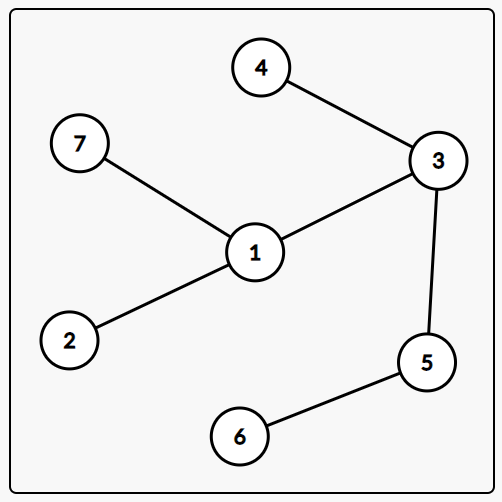
\includegraphics[scale=0.6]{graf}
\end{center}
Dari ilustrasi perumahan tersebut bisa didapat bahwa jarak kota-$1$ ke kota-$2$, kota-$3$, kota-$4$, kota-$5$, kota-$6$, kota-$7$ masing-masing secara berurutan adalah 1, 1, 2, 2, 3, dan 1.

\pagebreak

\end{document}